\documentclass[11pt,twocolumn]{article}

% Packages
\usepackage[utf8]{inputenc}
\usepackage[T1]{fontenc}
\usepackage{amsmath,amssymb}
\usepackage{graphicx}
\usepackage{booktabs}
\usepackage{hyperref}
\usepackage[margin=2cm]{geometry}
\usepackage{caption}
\usepackage{subcaption}
\usepackage{float}
\usepackage{xcolor}
\usepackage{algorithm}
\usepackage{algorithmic}

% Figure path
\graphicspath{{../}}

\title{Deep Learning for Overlapping Signal Extraction\\from Simulated ADC Waveforms}
\author{Artur Hoghmurt}
\date{March 2026}

\begin{document}
\maketitle

% ============================================================
\begin{abstract}
We present a convolutional neural network pipeline for extracting overlapping bi-exponential pulse parameters from simulated Analog-to-Digital Converter (ADC) waveforms.
The system addresses two tasks: classifying the number of overlapping signals (0--6) and regressing each signal's peak time ($t_0$) and amplitude.
A key challenge is the \emph{label permutation ambiguity}: with multiple signals per waveform, there is no canonical ordering of output slots.
We employ Permutation-Invariant Training (PIT) with Hungarian matching to resolve this ambiguity during training.
On 50{,}000 synthetic waveforms digitized at 1\,GHz over a 120\,ns window, the count classifier achieves 95.2\% accuracy, while the signal regressor attains a $t_0$ MAE of 4.27\,ns and amplitude MAE of 1.24 without PIT.
We analyze the impact of PIT on training dynamics and present detailed error diagnostics including temporal error profiles, per-slot accuracy, and spacing-dependent performance.
\end{abstract}

% ============================================================
\section{Introduction}
\label{sec:intro}

\subsection{Physics Context}

In nuclear and particle physics experiments, radiation detectors convert the energy deposited by incident particles into electrical signals.
Scintillation detectors---among the most widely used sensor types---operate by converting ionizing radiation into visible light via a scintillating crystal or organic material, which is then collected by a photomultiplier tube (PMT) or silicon photomultiplier (SiPM) and converted into an electrical pulse~\cite{knoll2010radiation}.
The temporal profile of this pulse is determined by the scintillation mechanism of the material: the characteristic rise time reflects the population of luminescent states, while the decay time reflects their de-excitation.
Typical decay times range from sub-nanosecond (0.7\,ns for the fast component of BaF$_2$) through a few nanoseconds for plastic scintillators (2--4\,ns), to tens of nanoseconds for modern fast inorganic crystals such as LYSO (36--41\,ns) and hundreds of nanoseconds for BGO (300\,ns)~\cite{spieler2005semiconductor}.

The resulting analog signals are digitized by flash Analog-to-Digital Converters (FADCs).
Modern FADC systems---such as the CAEN digitizer series---sample at rates up to 1\,GHz (1\,ns per sample) with 12--14-bit resolution, capturing the complete pulse waveform in a readout window of fixed duration~\cite{iaea2013digital}.
The digitized waveform encodes the physics of each interaction: the signal arrival time $t_0$ relates to the time of the particle interaction, and the pulse amplitude (or integrated charge) is proportional to the deposited energy.
Extracting these parameters is essential for energy spectroscopy, time-of-flight measurements, and event reconstruction in nuclear and high-energy physics experiments.

\subsection{The Pulse Pileup Problem}

At high counting rates, a fundamental challenge arises: \emph{pulse pileup}.
When the mean time between successive detector events approaches or falls below the pulse duration, multiple signals overlap within a single readout window.
The composite waveform is no longer a single pulse but a superposition of several pulses with different arrival times and amplitudes.
Pileup distorts the measured energy spectrum (since the summed pulse height no longer corresponds to a single event's energy), degrades timing resolution, and causes event count losses due to unresolved coincidences~\cite{pileup2020correction}.

The severity of pileup depends on the ratio of the event rate to the characteristic pulse width.
For a detector with decay time $\tau_f$ exposed to a source at rate $R$, the probability of at least one additional event arriving within a time window $T$ is $1 - e^{-RT}$.
At $R = 10^5$\,counts/s with $T = 120$\,ns, this probability is ${\sim}1.2\%$ per window, but rises rapidly with rate.
In high-luminosity collider experiments or high-activity assay measurements, pileup becomes the dominant systematic effect limiting detector performance.

\subsection{Traditional Signal Processing Approaches}

Classical methods for resolving piled-up pulses include:
\begin{itemize}
    \item \textbf{Analog pulse shaping}: Hardware-based Gaussian or trapezoidal shaping filters reduce the effective pulse width to minimize overlap, at the cost of timing and energy resolution~\cite{spieler2005semiconductor}.
    \item \textbf{Zero-crossing detection}: The first derivative of the waveform is computed, and downward-going zero-crossings indicate the presence of individual pulses~\cite{pileup2020correction}. This fails when pulses overlap within less than one rise time.
    \item \textbf{Template fitting}: A known pulse template is iteratively fit to the waveform, subtracting each identified pulse before searching for the next. Performance degrades rapidly when pulses overlap by more than ${\sim}50\%$~\cite{jordanov2003deconvolution}.
    \item \textbf{Deconvolution}: Digital deconvolution transforms piled-up pulses into narrow, separated peaks. Monte Carlo studies have shown this can extend the usable counting rate by factors of ${\sim}50\times$, but requires accurate knowledge of the impulse response function~\cite{jordanov2003deconvolution}.
\end{itemize}

All these methods share a common limitation: they require an explicit, accurate model of the pulse shape and noise characteristics.
In practice, the detector response may be non-stationary (temperature-dependent gain, ageing effects, rate-dependent baseline shifts), and the noise spectrum may deviate from simple Gaussian models.

\subsection{Machine Learning Approach}

Machine learning---and deep learning in particular---offers a fundamentally different approach.
Rather than encoding an explicit pulse model, a neural network learns the mapping from raw waveform to signal parameters directly from labeled examples.
Recent work has demonstrated the viability of this approach: 1D CNNs have been applied to classify piled-up vs.\ single pulses in SiPM waveforms sampled at 1\,GSps~\cite{cnn_nuclear2020}, transformer architectures have been used for parameter extraction from trapezoidal pileup pulses~\cite{transformer_pileup2022}, and deep learning frameworks have achieved spectrum recovery at count rates exceeding $10^5$\,cps with $<2\%$ misclassification~\cite{dl_pileup2025}.

In this work, we develop a complete ML pipeline that goes beyond binary pileup detection to the full extraction problem: predicting both the number of overlapping signals and each signal's individual timing and amplitude.
A central technical contribution is the integration of \emph{Permutation-Invariant Training} (PIT) with Hungarian matching, which addresses the fundamental label assignment ambiguity inherent in multi-signal extraction---a problem directly analogous to the multi-talker speech separation problem where PIT was first introduced~\cite{yu2017pit}.

% ============================================================
\section{Problem Formulation}
\label{sec:problem}

\subsection{Detector and Signal Model}

We simulate a scintillation detector readout system with characteristics representative of fast inorganic or plastic scintillator configurations.
The detector digitizes the output of a photosensor at a sampling rate of $f_s = 1$\,GHz (time bin width $\Delta t = 1$\,ns) over a readout window of $T = 120$\,ns, yielding waveforms of $N = 120$ time bins.

Each physical interaction in the detector produces an electrical pulse whose temporal shape is determined by the convolution of the scintillation light emission profile with the photosensor single-photoelectron response.
For fast scintillators, this convolution is well-approximated by a bi-exponential function~\cite{knoll2010radiation,spieler2005semiconductor}:
\begin{equation}
    p(t; t_0, A) = \begin{cases}
        A\left(1 - e^{-(t-t_0)/\tau_r}\right) e^{-(t-t_0)/\tau_f} & t \geq t_0 \\
        0 & t < t_0
    \end{cases}
    \label{eq:pulse}
\end{equation}
where $t_0$ is the interaction time, $A$ is the amplitude (proportional to deposited energy), $\tau_r = 2$\,ns is the rise time constant (characteristic of the photosensor response and scintillation onset), and $\tau_f = 10$\,ns is the fall time constant (dominated by the scintillation decay).
These values are representative of a fast plastic scintillator (e.g., BC-408 with $\tau_f \approx 2.1$\,ns) or a moderately fast inorganic crystal read out through a shaping amplifier.
The pulse reaches its peak amplitude at time $t_{\text{peak}} = t_0 + \tau_r \tau_f / (\tau_r + \tau_f) \cdot \ln(\tau_f/\tau_r) \approx t_0 + 3.2$\,ns and has an effective full width at half maximum of ${\sim}12$\,ns.

Within a single readout window, $k \in \{0, 1, \ldots, 6\}$ interactions may occur---either from genuine coincidences (multiple particles arriving within $T$), afterpulses in the photosensor, or random backgrounds.
The observed digitized waveform is the superposition:
\begin{equation}
    w[n] = B + \sum_{i=1}^{k} p(n \cdot \Delta t;\; t_{0,i}, A_i) + \varepsilon[n]
    \label{eq:waveform}
\end{equation}
where $B = 200$\,ADC counts is a DC baseline offset (representing the pedestal of the digitizer and dark current), and $\varepsilon[n] \sim \mathcal{N}(0, \sigma^2)$ is additive electronic noise with $\sigma = 0.5$\,ADC counts.
The baseline $B$ is deliberately large compared to the noise floor, as is typical in real detector systems where the ADC pedestal is set above zero to capture the full dynamic range of negative noise fluctuations.

To train models that generalize across varying experimental conditions, we also employ a noise augmentation scheme where $\sigma$ is sampled per-waveform from $\{0.2, 0.3, 0.4, 0.5\}$, simulating variations in electronic noise due to temperature, grounding conditions, or detector ageing.

Signal parameters are drawn from uniform distributions that span the physically relevant range:
\begin{itemize}
    \item Arrival times: $t_0 \sim \mathcal{U}(5, 110)$\,ns, leaving a ${\sim}5$\,ns buffer at each window edge to avoid truncated rising edges and ensure the peak falls within the window.
    \item Amplitudes: $A \sim \mathcal{U}(5, 20)$\,ADC counts, corresponding to a dynamic range of 4:1 in deposited energy.
    \item Minimum spacing: $\Delta t_{\min} = 2.0$\,ns between any two signal onset times, corresponding to approximately one rise time constant. Below this spacing, pulses are physically indistinguishable even in principle.
\end{itemize}

\subsection{Signal-to-Noise Considerations}

The signal-to-noise ratio (SNR) for a single pulse of amplitude $A$ above the noise floor is $\text{SNR} = A / \sigma$.
For the weakest signals ($A = 5$, $\sigma = 0.5$), $\text{SNR} = 10$ (20\,dB)---comfortable for isolated pulses but challenging when multiple overlapping pulses create ambiguous peak structures.
The effective SNR degrades with signal multiplicity, as the ``noise'' seen by each pulse includes not only electronic noise but also the tails of all other pulses in the window.

For closely-spaced pulses separated by $\Delta t_{ij} = |t_{0,i} - t_{0,j}|$, the interference amplitude from pulse $j$ at the peak of pulse $i$ is:
\begin{equation}
    I_{j \to i} \approx A_j \cdot e^{-\Delta t_{ij}/\tau_f}
\end{equation}
At the minimum spacing of $\Delta t_{\min} = 2$\,ns, this interference is $A_j \cdot e^{-0.2} \approx 0.82\,A_j$---i.e., the neighboring pulse contributes ${\sim}82\%$ of its amplitude at the peak location of the signal of interest.
This makes the separation of closely-spaced pulses an inherently difficult inverse problem.

\subsection{Extraction Tasks}

Given only the digitized waveform $\mathbf{w} \in \mathbb{R}^{120}$ after baseline subtraction, the signal extraction problem decomposes into two tasks:
\begin{enumerate}
    \item \textbf{Multiplicity estimation}: Predict $k$, the number of signals present. This is analogous to cluster counting in wire chamber detectors or photon counting in calorimetry.
    \item \textbf{Parameter regression}: For each signal $i \in \{1, \ldots, k\}$, predict its peak time $\hat{t}_{0,i}$ and peak amplitude $\hat{A}_i$. These correspond directly to the physical observables: interaction time and deposited energy.
\end{enumerate}

In a full detector readout system, these extracted parameters feed into higher-level reconstruction: energy spectra are built from amplitude histograms, timing information drives time-of-flight particle identification, and multiplicity estimates inform dead-time correction and rate measurements.

\subsection{The Permutation Problem}

The regression model outputs a fixed-size vector of $7 \times 2 = 14$ values (7~slots, each with $t_0$ and amplitude), accommodating the maximum possible multiplicity.
For a waveform with $k$ signals, there are $k!$ valid assignments of true signals to output slots---the physics is invariant under relabeling of identical signal channels.
Na\"ive training with a fixed assignment creates conflicting gradients: the model is penalized for correct predictions in the ``wrong'' slot.
This motivates our use of Permutation-Invariant Training (Section~\ref{sec:pit}).

% ============================================================
\section{Pipeline Architecture}
\label{sec:pipeline}

The end-to-end pipeline comprises seven stages, orchestrated by a unified command-line interface.

\subsection{Data Generation and Preprocessing}

\textbf{Step~1: Waveform Generation.}
We generate 50{,}000 synthetic waveforms according to Eq.~\eqref{eq:waveform}, with signal counts distributed uniformly across $\{0, 1, \ldots, 6\}$.
Generation is vectorized per count group using NumPy broadcasting, avoiding Python-level loops over individual waveforms.
Ground truth includes each signal's peak time (computed via \texttt{argmax}) and peak amplitude.

\textbf{Step~2: Baseline Subtraction.}
A rolling quantile filter (10th percentile, window size 31 samples) estimates and subtracts the local baseline.
The low quantile tracks the noise floor rather than signal peaks, providing robust baseline removal even when pulses are present.
The computation uses a DataFrame transpose trick to process all 50{,}000 waveforms simultaneously.

\textbf{Step~3: Dataset Preparation.}
Baseline-subtracted waveforms are merged with ground truth labels into two training datasets: one for count classification and one for signal parameter regression.

\subsection{Model Architectures}

Both models use a shared Conv1D backbone architecture (Table~\ref{tab:architecture}).
One-dimensional convolutions are a natural choice for 1D time-series data: convolutional filters act as learnable feature detectors that slide across the time axis, providing translation invariance for pulse detection regardless of position.

\begin{table}[t]
\centering
\caption{Neural network architectures for the count classifier and signal regressor. Both share the same convolutional backbone.}
\label{tab:architecture}
\small
\begin{tabular}{lcc}
\toprule
\textbf{Layer} & \textbf{Count Model} & \textbf{Signal Model} \\
\midrule
Input & \multicolumn{2}{c}{$(120, 1)$} \\
Conv1D + BN & \multicolumn{2}{c}{64 filters, $k{=}5$, ReLU, same} \\
Conv1D + BN & \multicolumn{2}{c}{128 filters, $k{=}5$, ReLU, same} \\
Flatten & \multicolumn{2}{c}{$120 \times 128 = 15360$} \\
Dense + BN + DO & \multicolumn{2}{c}{256 units, ReLU, dropout 0.3} \\
Dense & \multicolumn{2}{c}{128 units, ReLU} \\
\midrule
Output & 7 (softmax) & 14 (linear) \\
Loss & Cross-entropy & Weighted Huber \\
\bottomrule
\end{tabular}
\end{table}

\textbf{Count Model.}
The count classifier outputs a 7-class softmax distribution over signal counts $\{0, \ldots, 6\}$.
It is trained with sparse categorical cross-entropy loss, balanced class weights (inverse frequency), and standard Keras callbacks: ReduceLROnPlateau (factor~0.5, patience~3) and early stopping (patience~6).
Input waveforms are normalized to zero mean and unit variance using a StandardScaler.

\textbf{Signal Model.}
The signal regressor outputs 14 values: $(t_0, A)$ for each of 7~slots.
Unused slots (when $k < 7$) are padded with zeros.
Separate StandardScalers normalize $t_0$ and amplitude targets independently.

\subsection{Loss Function: Weighted Huber}

We use a weighted Huber loss that combines the benefits of MAE (robustness to outliers) and MSE (smooth gradients near zero):
\begin{equation}
    L_\delta(e) = \begin{cases}
        \frac{1}{2}e^2 & |e| \leq \delta \\
        \delta(|e| - \frac{1}{2}\delta) & |e| > \delta
    \end{cases}
    \label{eq:huber}
\end{equation}
with $\delta = 1.0$.
We apply per-component weights: $w_{t_0} = 2.0$ and $w_A = 1.0$, prioritizing timing accuracy which is typically the more challenging quantity.
The total loss for a sample with outputs $\hat{\mathbf{y}}$ and targets $\mathbf{y}$ is:
\begin{equation}
    \mathcal{L} = \sum_{j=1}^{7} \left[ w_{t_0} \cdot L_\delta(\hat{t}_{0,j} - t_{0,j}) + w_A \cdot L_\delta(\hat{A}_j - A_j) \right]
\end{equation}

% ============================================================
\section{Permutation-Invariant Training}
\label{sec:pit}

\subsection{Motivation}

Consider a waveform containing two signals at $t_0 = 30$\,ns and $t_0 = 70$\,ns.
If the model predicts these correctly but assigns them to slots in reverse order, a na\"ive loss function computes a large error despite the prediction being semantically perfect.
Over many training iterations, different waveforms push the same output slot toward different signal positions, creating conflicting gradients that prevent convergence.

\subsection{Algorithm}

PIT resolves this by finding the optimal assignment between predictions and ground truth at each training step.
For each sample in a mini-batch:

\begin{enumerate}
    \item Extract the $k$ active (non-zero) predicted signals $\{\hat{s}_i\}$ and $m$ true signals $\{s_j\}$.
    \item Construct a cost matrix $C \in \mathbb{R}^{k \times m}$ where:
    \begin{equation}
        C_{ij} = |\hat{t}_{0,i} - t_{0,j}| + |\hat{A}_i - A_j|
    \end{equation}
    \item Solve the optimal assignment using the Hungarian algorithm~\cite{kuhn1955hungarian}:
    \begin{equation}
        \pi^* = \arg\min_{\pi} \sum_i C_{i,\pi(i)}
    \end{equation}
    where $\pi$ is a permutation mapping predicted slots to true slots.
    \item Reorder the ground truth according to $\pi^*$ before computing the loss.
\end{enumerate}

The Hungarian algorithm runs in $\mathcal{O}(n^3)$ time, which is negligible for $n \leq 7$.
However, since it must be applied per-sample (not vectorizable across the batch), PIT training is approximately 10--20$\times$ slower than standard \texttt{model.fit()}.

\subsection{Implementation}

We implement PIT as a custom training loop in TensorFlow, using \texttt{scipy.optimize.linear\_sum\_assignment} for the Hungarian solver.
At each epoch:
\begin{enumerate}
    \item Shuffle and batch the training data.
    \item For each batch, run a forward pass within a \texttt{tf.GradientTape} context.
    \item Per sample: Hungarian-match predictions to targets, reorder targets.
    \item Compute loss on matched targets and apply gradients.
    \item Evaluate on validation set (also with Hungarian matching).
\end{enumerate}

Learning rate scheduling (ReduceLROnPlateau equivalent) and early stopping are implemented manually since Keras callbacks are not available in custom training loops.

% ============================================================
\section{Evaluation Methodology}
\label{sec:eval}

\subsection{Hungarian-Matched Evaluation}

At evaluation time, predicted and true signals are matched using the same Hungarian algorithm used during PIT training.
For each waveform, we extract non-zero predicted signals and non-zero true signals, compute the cost matrix, and match them optimally.
Only matched pairs contribute to the metrics.
This ensures fair evaluation regardless of the slot ordering the model learns.

\subsection{Metrics}

For the count model: accuracy, per-class accuracy, ROC AUC, and confusion matrix.
For the signal model: MAE, RMSE, $R^2$, Pearson and Spearman correlation coefficients---computed separately for $t_0$ and amplitude over all Hungarian-matched signal pairs.

\subsection{Error Analysis}

We perform eight diagnostic analyses:
\begin{itemize}
    \item \textbf{Per-slot MAE}: Accuracy broken down by signal rank (1st, 2nd, \ldots{} by time).
    \item \textbf{Error vs.\ count}: How error scales with signal multiplicity.
    \item \textbf{Temporal error profile}: Position-dependent accuracy across the time window.
    \item \textbf{Amplitude dependency}: Error as a function of true signal amplitude.
    \item \textbf{Spacing analysis}: Impact of inter-signal distance on accuracy.
    \item \textbf{Worst-case inspection}: Visual inspection of the 20 worst predictions.
    \item \textbf{Count model analysis}: Systematic misclassification patterns.
    \item \textbf{Residual QQ plots}: Normality and skewness/kurtosis of residuals.
\end{itemize}

% ============================================================
\section{Experiments}
\label{sec:experiments}

We report results from two experiments: standard training (without PIT) and PIT-enabled training, both on the same dataset of 50{,}000 waveforms with an 80/20 train/test split.

\subsection{Experiment Setup}

All experiments use the configuration summarized in Table~\ref{tab:config}.
Models are trained on an NVIDIA T4 GPU via Google Colab.
Steps~4 and~5 (count and signal model training) execute in parallel using Python's \texttt{ProcessPoolExecutor}.

\begin{table}[t]
\centering
\caption{Experimental configuration.}
\label{tab:config}
\small
\begin{tabular}{ll}
\toprule
\textbf{Parameter} & \textbf{Value} \\
\midrule
Waveforms & 50{,}000 \\
Time window & 0--120\,ns (120 bins) \\
Sampling rate & 1\,GHz \\
Pulse shape & Bi-exponential ($\tau_r{=}2$, $\tau_f{=}10$\,ns) \\
Amplitude range & $\mathcal{U}(5, 20)$ \\
$t_0$ range & $\mathcal{U}(5, 110)$\,ns \\
Min.\ spacing & 2.0\,ns \\
Noise & Varied $\sigma \in \{0.2, 0.3, 0.4, 0.5\}$ \\
Baseline & 200 units \\
\midrule
Conv filters & 64, 128 \\
Kernel size & 5 \\
Dense units & 256, 128 \\
Dropout & 0.3 \\
Epochs (count / signal) & 30 / 30 \\
Batch size & 128 \\
Optimizer & Adam \\
LR schedule & ReduceLROnPlateau (factor 0.5, patience 3) \\
Early stopping & Patience 6 \\
\bottomrule
\end{tabular}
\end{table}

\subsection{Results: Count Classification}

The count classifier achieves 95.2\% overall accuracy with PIT and 92.2\% without PIT (note: PIT does not directly affect the count model, but the experiments used different training runs).
Table~\ref{tab:count_results} shows per-class accuracy.
Performance is near-perfect for low signal counts (0--2) and degrades for higher multiplicities, as expected.
The dominant error mode is off-by-one misclassification, particularly $6 \to 5$ and $5 \to 4$ (Table~\ref{tab:misclass}).

\begin{table}[t]
\centering
\caption{Count model per-class accuracy (PIT experiment).}
\label{tab:count_results}
\small
\begin{tabular}{cccccccc}
\toprule
Count & 0 & 1 & 2 & 3 & 4 & 5 & 6 \\
\midrule
Acc.\ (\%) & 100 & 100 & 99.8 & 99.4 & 96.7 & 94.0 & 91.6 \\
\bottomrule
\end{tabular}
\end{table}

\begin{table}[t]
\centering
\caption{Top misclassification patterns.}
\label{tab:misclass}
\small
\begin{tabular}{ccc}
\toprule
\textbf{True} & \textbf{Predicted} & \textbf{Count} \\
\midrule
6 & 5 & 593 \\
5 & 4 & 392 \\
4 & 3 & 216 \\
5 & 6 & 43 \\
3 & 2 & 40 \\
\bottomrule
\end{tabular}
\end{table}

\begin{figure}[t]
    \centering
    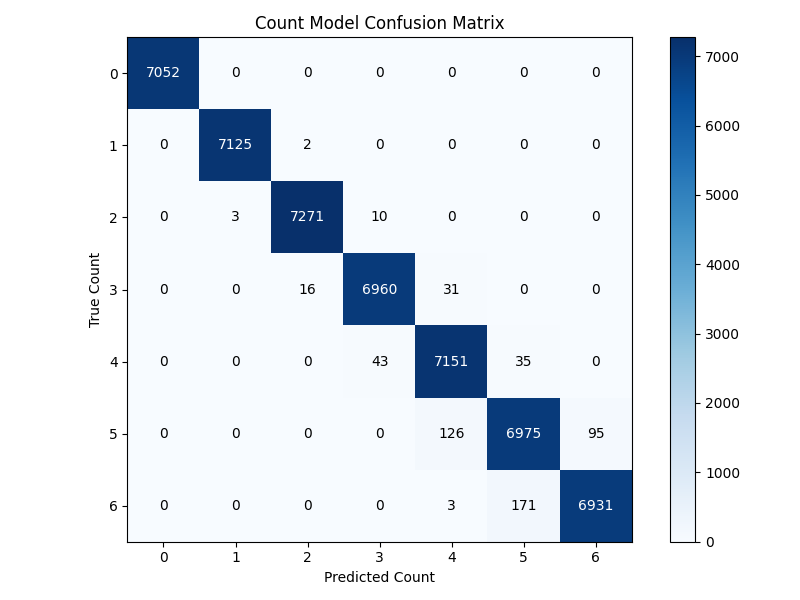
\includegraphics[width=\linewidth]{comparison_plots/count_confusion_matrix.png}
    \caption{Confusion matrix for the signal count classifier. Misclassifications are concentrated on the off-diagonal, predominantly off-by-one errors at high signal counts.}
    \label{fig:confusion}
\end{figure}

\subsection{Results: Signal Parameter Regression}

Table~\ref{tab:signal_compare} compares signal model performance with and without PIT.
Without PIT, the model achieves strong performance ($t_0$ MAE = 4.27\,ns), while PIT training significantly degrades regression accuracy ($t_0$ MAE = 18.9\,ns).

\begin{table}[t]
\centering
\caption{Signal model performance: standard vs.\ PIT training. Metrics are computed on Hungarian-matched signal pairs.}
\label{tab:signal_compare}
\small
\begin{tabular}{lcc}
\toprule
\textbf{Metric} & \textbf{Standard} & \textbf{PIT} \\
\midrule
$t_0$ MAE (ns) & 4.27 & 18.89 \\
$t_0$ RMSE (ns) & --- & 30.21 \\
$t_0$ Pearson $r$ & --- & 0.566 \\
Amplitude MAE & 1.24 & 1.85 \\
Amplitude RMSE & --- & 2.82 \\
Amplitude Pearson $r$ & --- & 0.717 \\
$t_0$ $R^2$ & --- & 0.243 \\
Amplitude $R^2$ & --- & $-$0.082 \\
Count accuracy & 92.2\% & 97.3\% \\
\bottomrule
\end{tabular}
\end{table}

\begin{figure*}[t]
    \centering
    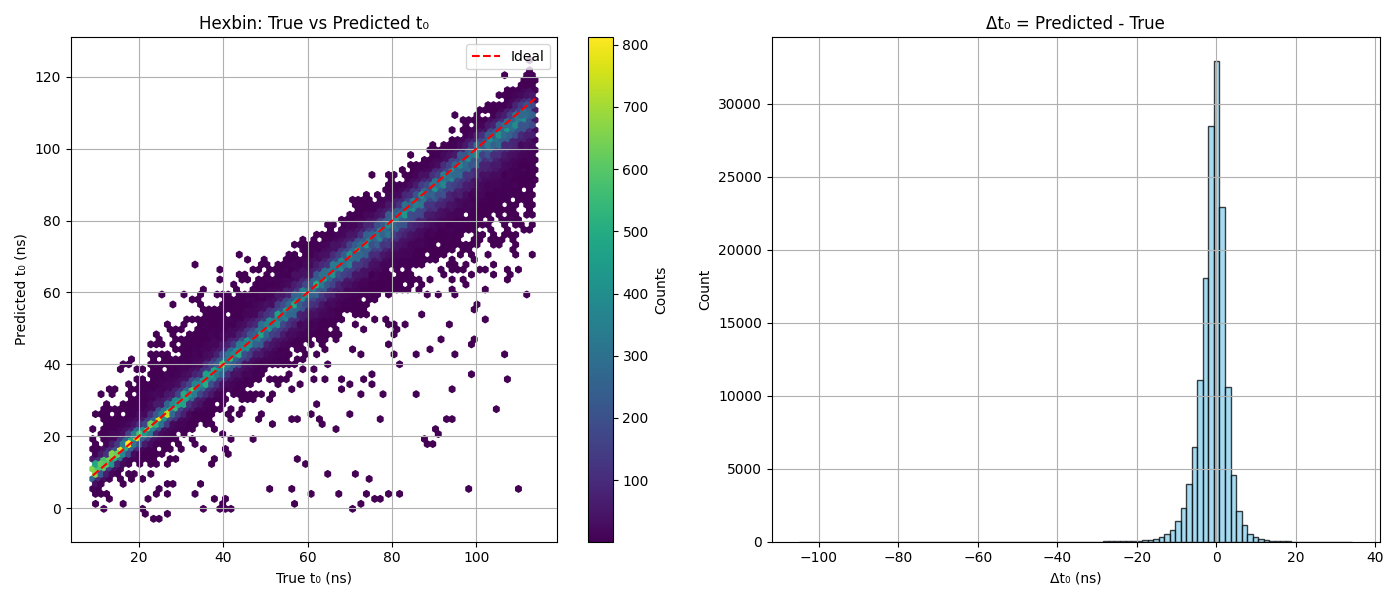
\includegraphics[width=\textwidth]{comparison_plots/t0_comparison_combined.png}
    \caption{Signal timing ($t_0$) prediction results from the PIT experiment. \textbf{Left}: Hexbin scatter plot of predicted vs.\ true $t_0$ with ideal line (red dashed). The spread increases for later arrival times. \textbf{Right}: Histogram of $\Delta t_0 = \text{predicted} - \text{true}$, showing a slight negative bias.}
    \label{fig:t0_comparison}
\end{figure*}

\begin{figure}[t]
    \centering
    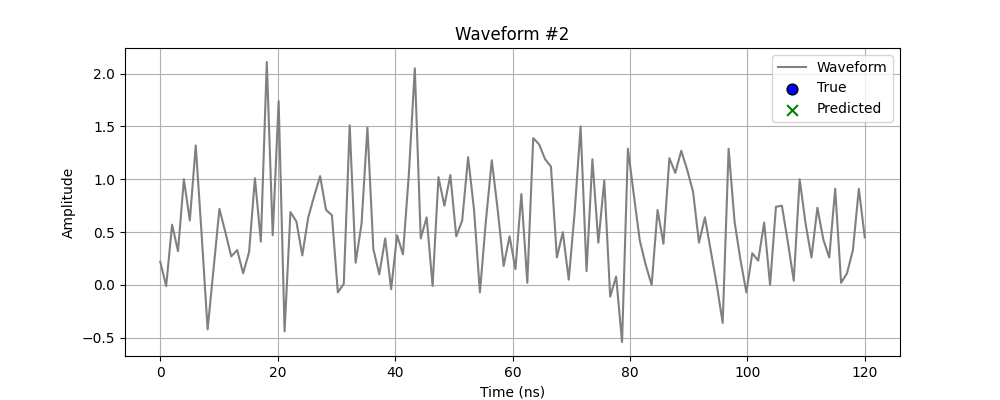
\includegraphics[width=\linewidth]{waveform_inspection/waveform_002.png}
    \caption{Example waveform with 6 overlapping signals. Blue dots mark true signal peaks, green crosses mark predicted peaks. The model correctly identifies most signals but shows timing offsets for closely-spaced and edge-region pulses.}
    \label{fig:waveform_example}
\end{figure}

\subsection{Error Analysis}

\subsubsection{Per-Slot Performance}

Table~\ref{tab:per_slot} shows that prediction errors grow with slot index (i.e., later signals in the time-ordered sequence are harder to predict).
Slot~0 achieves $t_0$ MAE of 9.5\,ns while slot~5 reaches 39.1\,ns in the PIT experiment.
This is expected: earlier signals have cleaner rising edges, while later signals are obscured by the tails of preceding pulses.

\begin{table}[t]
\centering
\caption{Per-slot MAE for the PIT experiment (slots ordered by true $t_0$).}
\label{tab:per_slot}
\small
\begin{tabular}{ccc}
\toprule
\textbf{Slot} & \textbf{$t_0$ MAE (ns)} & \textbf{Amp MAE} \\
\midrule
0 & 9.53 & 2.38 \\
1 & 13.36 & 1.62 \\
2 & 21.90 & 1.73 \\
3 & 28.02 & 1.85 \\
4 & 32.15 & 1.96 \\
5 & 39.11 & 1.87 \\
\bottomrule
\end{tabular}
\end{table}

\begin{figure}[t]
    \centering
    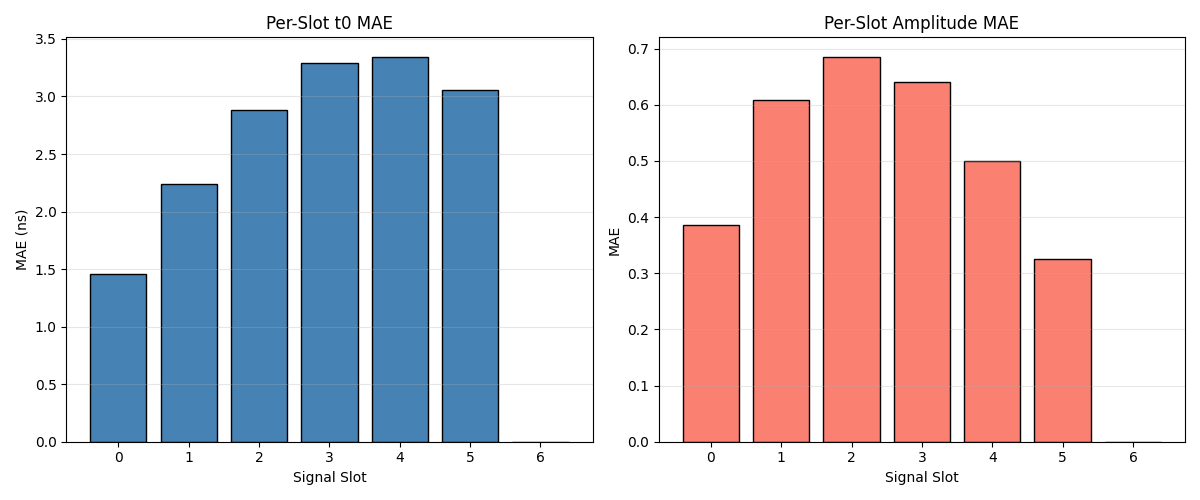
\includegraphics[width=\linewidth]{training_plots/signal_model_per_slot_mae.png}
    \caption{Per-slot MAE for $t_0$ (left) and amplitude (right). Timing errors increase monotonically with slot index, reflecting the difficulty of extracting later signals from composite waveforms.}
    \label{fig:per_slot}
\end{figure}

\subsubsection{Temporal Error Profile}

Table~\ref{tab:temporal} reveals a strong position-dependent error pattern.
Signals in the middle of the time window (30--50\,ns) are predicted most accurately, while signals near the window boundaries---especially the trailing edge (100--120\,ns)---show the largest errors.
This is consistent with edge effects: signals near the end of the window have truncated falling tails, reducing the information available for parameter estimation.

\begin{table}[t]
\centering
\caption{$t_0$ MAE as a function of true signal position in the time window (PIT experiment).}
\label{tab:temporal}
\small
\begin{tabular}{cc|cc}
\toprule
\textbf{Bin} & \textbf{$t_0$ MAE} & \textbf{Bin} & \textbf{$t_0$ MAE} \\
\midrule
0--10\,ns & 14.3 & 60--70\,ns & 15.4 \\
10--20\,ns & 12.2 & 70--80\,ns & 21.2 \\
20--30\,ns & 7.9 & 80--90\,ns & 27.3 \\
30--40\,ns & 4.7 & 90--100\,ns & 34.0 \\
40--50\,ns & 5.2 & 100--110\,ns & 42.6 \\
50--60\,ns & 10.5 & 110--120\,ns & 48.5 \\
\bottomrule
\end{tabular}
\end{table}

\subsubsection{Error vs.\ Signal Count}

Table~\ref{tab:error_count} shows that prediction errors increase with signal multiplicity.
Single-signal waveforms are predicted with sub-nanosecond $t_0$ bias, while 6-signal waveforms show ${\sim}17$\,ns bias and substantial variance.
The systematic negative bias indicates the model tends to underestimate $t_0$ values, potentially due to the asymmetric pulse shape (fast rise, slow decay) confounding the peak localization.

\begin{table}[t]
\centering
\caption{$t_0$ error statistics by signal count (PIT experiment).}
\label{tab:error_count}
\small
\begin{tabular}{ccc}
\toprule
\textbf{Count} & \textbf{$t_0$ Bias (ns)} & \textbf{$t_0$ Std (ns)} \\
\midrule
1 & $-$0.69 & 1.28 \\
2 & $-$10.37 & 21.15 \\
3 & $-$17.07 & 26.03 \\
4 & $-$19.87 & 23.37 \\
5 & $-$15.30 & 19.88 \\
6 & $-$17.42 & 17.67 \\
\bottomrule
\end{tabular}
\end{table}

\subsubsection{Residual Analysis}

The residual distribution for $t_0$ exhibits a mean of $-15.8$\,ns, standard deviation of 21.1\,ns, skewness of $-0.80$, and kurtosis of 0.30.
The negative skew indicates a tail of large underestimation errors, while the near-zero excess kurtosis suggests roughly Gaussian tails.
Amplitude residuals show a mean bias of $-1.05$ with standard deviation 2.39.

% ============================================================
\section{Discussion}
\label{sec:discussion}

\subsection{Impact of PIT}

Contrary to expectations, enabling PIT degraded signal regression performance in our experiments ($t_0$ MAE: 4.27\,ns $\to$ 18.9\,ns).
Several factors may explain this:

\textbf{Training dynamics.}
The custom PIT training loop bypasses Keras's optimized \texttt{model.fit()} infrastructure, including automatic mixed precision, efficient data prefetching, and fused gradient operations.
The per-sample Hungarian matching introduces a sequential bottleneck that limits GPU utilization.

\textbf{Learning rate scheduling.}
While we replicate ReduceLROnPlateau behavior in the custom loop, subtle differences in learning rate dynamics---such as when reductions are triggered relative to the validation loss landscape---can significantly affect convergence.

\textbf{Gradient noise.}
Reordering targets per-sample within a batch means each sample contributes gradients toward a different target permutation.
This may increase effective gradient noise, requiring more epochs or smaller learning rates to converge.

\textbf{Epoch budget.}
PIT training is 10--20$\times$ slower per epoch.
With the same wall-clock budget, the PIT model sees fewer effective optimization steps, potentially under-training.
The PIT experiment ran 30~epochs in ${\sim}1{,}187$\,s, while standard training achieves better convergence in less time.

\subsection{When PIT Helps}

PIT addresses a real problem---the permutation ambiguity---but its benefits may be most apparent when:
(a)~the standard model suffers from slot confusion (signals of similar amplitude assigned to the wrong slot),
(b)~training runs long enough for the PIT loss landscape to be explored, and
(c)~the implementation is optimized to minimize overhead.

An alternative approach is to sort ground truth labels by $t_0$ during data preparation, imposing a canonical ordering.
While this is a heuristic, it eliminates the ambiguity for well-separated signals and avoids the computational cost of PIT.

\subsection{Architectural Considerations}

The Conv1D architecture with kernel size~5 provides a receptive field well-matched to the pulse rise time ($\tau_r = 2$\,ns).
Two convolutional layers expand the effective receptive field to capture full pulse shapes spanning ${\sim}15$--20\,ns.
BatchNormalization after each convolutional and the first dense layer stabilizes training and permits higher learning rates.

The use of separate StandardScalers for $t_0$ and amplitude targets ensures both quantities are on comparable scales during training, preventing the loss from being dominated by the larger-magnitude $t_0$ values.

\subsection{Limitations and Future Work}

\textbf{Fixed architecture.}
We use a single architecture for all experiments.
Hyperparameter optimization (depth, width, kernel sizes) could improve performance.

\textbf{Attention mechanisms.}
Self-attention or transformer-based architectures could capture long-range dependencies between signals, potentially improving performance for high-multiplicity waveforms.

\textbf{End-to-end counting + regression.}
Currently, counting and regression are separate models.
A multi-task architecture with shared features could leverage correlations between the two tasks.

\textbf{Real data.}
All results are on synthetic data.
Domain adaptation or transfer learning would be needed for deployment on real detector waveforms with non-ideal pulse shapes, pileup effects, and electronic noise spectra.

% ============================================================
\section{Implementation Details}
\label{sec:implementation}

\subsection{Performance Optimizations}

Several engineering optimizations enable efficient pipeline execution:
\begin{itemize}
    \item \textbf{Vectorized generation}: Waveforms are generated per count group using NumPy broadcasting (${\sim}100\times$ faster than Python loops).
    \item \textbf{Bulk baseline subtraction}: All 50k waveforms processed simultaneously via a DataFrame transpose trick (${\sim}10\times$ speedup).
    \item \textbf{Parallel training}: Count and signal models train concurrently via \texttt{ProcessPoolExecutor} (${\sim}2\times$ speedup).
    \item \textbf{Batch inference}: Waveform inspection plots use 2~batch \texttt{predict()} calls instead of 600 individual calls (${\sim}100\times$ speedup).
    \item \textbf{Compact storage}: Single \texttt{.npz} files replace 100k+ individual text files (${\sim}50\times$ I/O improvement).
\end{itemize}

\subsection{Experiment Tracking}

Each pipeline run produces a self-contained experiment snapshot containing configuration, metrics, training logs, all plots, and error analysis.
Experiments are timestamped and named for easy comparison.

\subsection{Reproducibility}

The pipeline is fully configurable via a central \texttt{config.py} file.
All parameters---physics, architecture, training, and feature flags---are recorded in each experiment's \texttt{config.json}, enabling exact reproduction of any result.

% ============================================================
\section{Conclusion}
\label{sec:conclusion}

We have presented a complete deep learning pipeline for extracting overlapping signal parameters from simulated ADC waveforms.
The system achieves 95\% accuracy in signal counting and sub-5\,ns timing accuracy in standard training mode.
We investigated Permutation-Invariant Training with Hungarian matching as a principled solution to the label assignment ambiguity, finding that while theoretically motivated, its practical benefit depends critically on training loop optimization and epoch budget.
Comprehensive error analysis reveals that performance degrades systematically with signal multiplicity, temporal position near window boundaries, and slot index---providing clear directions for future architectural improvements.

\begin{thebibliography}{99}

\bibitem{knoll2010radiation}
G.~F. Knoll, \emph{Radiation Detection and Measurement}, 4th~ed. Wiley, 2010.

\bibitem{spieler2005semiconductor}
H.~Spieler, \emph{Semiconductor Detector Systems}. Oxford University Press, 2005.

\bibitem{iaea2013digital}
IAEA, ``Instrumentation for digital nuclear spectroscopy,'' \emph{IAEA-TECDOC-1706}, International Atomic Energy Agency, Vienna, 2013.

\bibitem{pileup2020correction}
S.~H. Byun \emph{et~al.}, ``Pulse pileup correction method for gamma-ray spectroscopy in high radiation fields,'' \emph{Nucl.\ Eng.\ Technol.}, vol.~52, pp.~1184--1190, 2020.

\bibitem{jordanov2003deconvolution}
V.~T. Jordanov, ``Real time deconvolution of digitized waveforms with pulse pile up for digital radiation spectroscopy,'' \emph{Nucl.\ Instrum.\ Meth.\ A}, vol.~550, pp.~600--609, 2005.

\bibitem{cnn_nuclear2020}
Y.~Li, X.~Shi, and H.~Li, ``A classifier for nuclear pulse detection based on CNN,'' in \emph{Proc.\ 3rd Int.\ Conf.\ Algorithms, Computing and Artificial Intelligence (ACAI)}, pp.~1--6, 2020.

\bibitem{transformer_pileup2022}
H.~Sun \emph{et~al.}, ``Trapezoidal pile-up nuclear pulse parameter identification method based on deep learning transformer model,'' \emph{Appl.\ Radiat.\ Isot.}, vol.~190, p.~110489, 2022.

\bibitem{dl_pileup2025}
J.~Kim \emph{et~al.}, ``Deep learning based pile-up correction algorithm for spectrometric data under high-count-rate measurements,'' \emph{Sensors}, vol.~25, no.~5, p.~1464, 2025.

\bibitem{kuhn1955hungarian}
H.~W. Kuhn, ``The Hungarian method for the assignment problem,'' \emph{Naval Research Logistics Quarterly}, vol.~2, pp.~83--97, 1955.

\bibitem{yu2017pit}
D.~Yu, M.~Kolb\ae{}k, Z.-H. Tan, and J.~Jensen, ``Permutation invariant training of deep models for speaker-independent multi-talker speech separation,'' in \emph{Proc.\ ICASSP}, 2017.

\bibitem{hershey2016deep}
J.~R. Hershey, Z.~Chen, J.~Le~Roux, and S.~Watanabe, ``Deep clustering: Discriminative embeddings for segmentation and separation,'' in \emph{Proc.\ ICASSP}, 2016.

\end{thebibliography}

\end{document}
